\documentclass[t]{beamer}   % base slides class

\usepackage[utf8]{inputenc} % to be able to type unicode text directly
\usepackage{graphicx}       % to include figures
\usepackage{animate}        % to include animations
%\usepackage{hyperref,url}   % to make clickable hyperlinks
%\usepackage{minted}         % for code insets



% disable useless beamer buttons
\mode<all>\setbeamertemplate{navigation symbols}{}

% set slide numbers in green
\mode<presentation>\defbeamertemplate*{footline}{infoline theme}
{\leavevmode\hfill\color{black!50!green}
	\insertframenumber{} / \inserttotalframenumber\hspace*{2ex}
\vskip0pt}





\begin{document}

\begin{frame}
A Gaussian volcano:
\[
	u(x,y)
	=
	200
	\left( 1+\tfrac13 x \right)
	\left(
		\tfrac{13}{10}e^{-10\left(x^2+y^2\right)}
		-e^{-20\left(x^2+y^2\right)}
	\right)
\]

Direct shading model~{\color{gray}[1]}:
\[
	I(x,y) = \left({
		{\color{red}\alpha}u_x
		+
		{\color{red}\beta}u_y
		+
		{\color{red}\gamma}
}\right)/{\sqrt{u_x^2+u_y^2+1}}
\]

\vfill

\begin{tabular}{cc}
	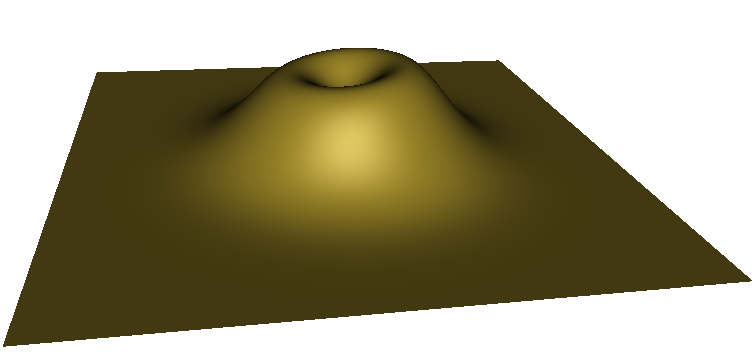
\includegraphics[width=0.5\linewidth]{f/volcano3d.png} &
	%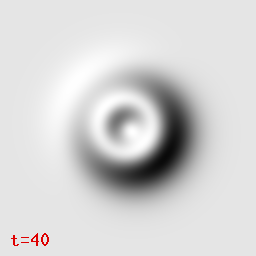
\includegraphics[width=0.25\linewidth]{f/cview_4.png} \\
	\animategraphics[width=0.25\linewidth,loop,autoplay]{4}{f/cview_}{1}{36} \\
	$z=u(x,y)$ &
	$I(x,y)$ \\
	&
	\tiny
	$({\color{red}\alpha},{\color{red}\beta})
	=
	(\cos{\color{red}t},\sin{\color{red}t})$
\end{tabular}

\vfill

{
	\tiny
	\color{gray}
	[1] Horn-Brooks,
	\emph{The variational approach to shape form shading},
	1986
}

\end{frame}



\end{document}
